\documentclass[journal,12pt,twocolumn]{IEEEtran}

\usepackage{setspace}
\usepackage{gensymb}
\singlespacing
\usepackage[cmex10]{amsmath}

\usepackage{amsthm}

\usepackage{mathrsfs}
\usepackage{txfonts}
\usepackage{stfloats}
\usepackage{bm}
\usepackage{cite}
\usepackage{cases}
\usepackage{subfig}
\usepackage{tikz}
\usepackage{longtable}
\usepackage{multirow}

\usepackage{enumitem}
\usepackage{mathtools}
\usepackage{steinmetz}
\usepackage{tikz}
\usepackage{circuitikz}
\usepackage{verbatim}
\usepackage{tfrupee}
\usepackage[breaklinks=true]{hyperref}
\usepackage{graphicx}
\usepackage{tkz-euclide}

\usetikzlibrary{calc,math}
\usepackage{listings}
    \usepackage{color}                                            %%
    \usepackage{array}                                            %%
    \usepackage{longtable}                                        %%
    \usepackage{calc}                                             %%
    \usepackage{multirow}                                         %%
    \usepackage{hhline}                                           %%
    \usepackage{ifthen}                                           %%
    \usepackage{lscape}     
\usepackage{multicol}
\usepackage{chngcntr}

\DeclareMathOperator*{\Res}{Res}

\renewcommand\thesection{\arabic{section}}
\renewcommand\thesubsection{\thesection.\arabic{subsection}}
\renewcommand\thesubsubsection{\thesubsection.\arabic{subsubsection}}

\renewcommand\thesectiondis{\arabic{section}}
\renewcommand\thesubsectiondis{\thesectiondis.\arabic{subsection}}
\renewcommand\thesubsubsectiondis{\thesubsectiondis.\arabic{subsubsection}}


\hyphenation{op-tical net-works semi-conduc-tor}
\def\inputGnumericTable{}                                 %%

\lstset{
%language=C,
frame=single, 
breaklines=true,
columns=fullflexible
}
\begin{document}


\newtheorem{theorem}{Theorem}[section]
\newtheorem{problem}{Problem}
\newtheorem{proposition}{Proposition}[section]
\newtheorem{lemma}{Lemma}[section]
\newtheorem{corollary}[theorem]{Corollary}
\newtheorem{example}{Example}[section]
\newtheorem{definition}[problem]{Definition}

\newcommand{\BEQA}{\begin{eqnarray}}
\newcommand{\EEQA}{\end{eqnarray}}
\newcommand{\define}{\stackrel{\triangle}{=}}
\bibliographystyle{IEEEtran}
\raggedbottom
\setlength{\parindent}{0pt}
\providecommand{\mbf}{\mathbf}
\providecommand{\pr}[1]{\ensuremath{\Pr\left(#1\right)}}
\providecommand{\qfunc}[1]{\ensuremath{Q\left(#1\right)}}
\providecommand{\sbrak}[1]{\ensuremath{{}\left[#1\right]}}
\providecommand{\lsbrak}[1]{\ensuremath{{}\left[#1\right.}}
\providecommand{\rsbrak}[1]{\ensuremath{{}\left.#1\right]}}
\providecommand{\brak}[1]{\ensuremath{\left(#1\right)}}
\providecommand{\lbrak}[1]{\ensuremath{\left(#1\right.}}
\providecommand{\rbrak}[1]{\ensuremath{\left.#1\right)}}
\providecommand{\cbrak}[1]{\ensuremath{\left\{#1\right\}}}
\providecommand{\lcbrak}[1]{\ensuremath{\left\{#1\right.}}
\providecommand{\rcbrak}[1]{\ensuremath{\left.#1\right\}}}
\theoremstyle{remark}
\newtheorem{rem}{Remark}
\newcommand{\sgn}{\mathop{\mathrm{sgn}}}
% \providecommand{\abs}[1]{\left\vert#1\right\vert}
% \providecommand{\res}[1]{\Res\displaylimits_{#1}} 
% \providecommand{\norm}[1]{\left\lVert#1\right\rVert}
% %\providecommand{\norm}[1]{\lVert#1\rVert}
% \providecommand{\mtx}[1]{\mathbf{#1}}
% \providecommand{\mean}[1]{E\left[ #1 \right]}
\providecommand{\fourier}{\overset{\mathcal{F}}{ \rightleftharpoons}}
%\providecommand{\hilbert}{\overset{\mathcal{H}}{ \rightleftharpoons}}
\providecommand{\system}{\overset{\mathcal{H}}{ \longleftrightarrow}}
	%\newcommand{\solution}[2]{\textbf{Solution:}{#1}}
\newcommand{\solution}{\noindent \textbf{Solution: }}
\newcommand{\cosec}{\,\text{cosec}\,}
\providecommand{\dec}[2]{\ensuremath{\overset{#1}{\underset{#2}{\gtrless}}}}
\newcommand{\myvec}[1]{\ensuremath{\begin{pmatrix}#1\end{pmatrix}}}
\newcommand{\mydet}[1]{\ensuremath{\begin{vmatrix}#1\end{vmatrix}}}
\numberwithin{equation}{subsection}
\def\putbox#1#2#3{\makebox[0in][l]{\makebox[#1][l]{}\raisebox{\baselineskip}[0in][0in]{\raisebox{#2}[0in][0in]{#3}}}}
     \def\rightbox#1{\makebox[0in][r]{#1}}
     \def\centbox#1{\makebox[0in]{#1}}
     \def\topbox#1{\raisebox{-\baselineskip}[0in][0in]{#1}}
     \def\midbox#1{\raisebox{-0.5\baselineskip}[0in][0in]{#1}}
\vspace{3cm}
\title{Assignment 1}
\author{Aayush Goyal - EE18BTECH11001}
\maketitle
\newpage
\bigskip
Github repository
%
\begin{lstlisting}
https://github.com/aayush2710/EE4013-Assignment1
\end{lstlisting}
\setcounter{figure}{0}
\section{Problem}
Consider the following Recurrence Relation
\begin{multline}
  T(n) =
  \begin{cases}
  T(n/2) + T(2n/5) + 7n & \text{if } n>0 \\
  1 & \text{if } n=0
  \end{cases}
\end{multline}

Which one of the following options is correct?
\begin{enumerate}
    \item $T(n) = \mathcal{O}(n^{\frac{5}{2}})$
    \item $T(n) = \mathcal{O}(n\log n)$
    \item $T(n) = \mathcal{O}(n)$
    \item $T(n) = \mathcal{O}((\log n)^{\frac{5}{2}})$
\end{enumerate}
\section{Solution}
We need to calculate the worst case time complexity of the given recurrence relation.
\\
Let us start by drawing the recurrence tree for the given problem. 
\\
\begin{figure}[!h]
\centering
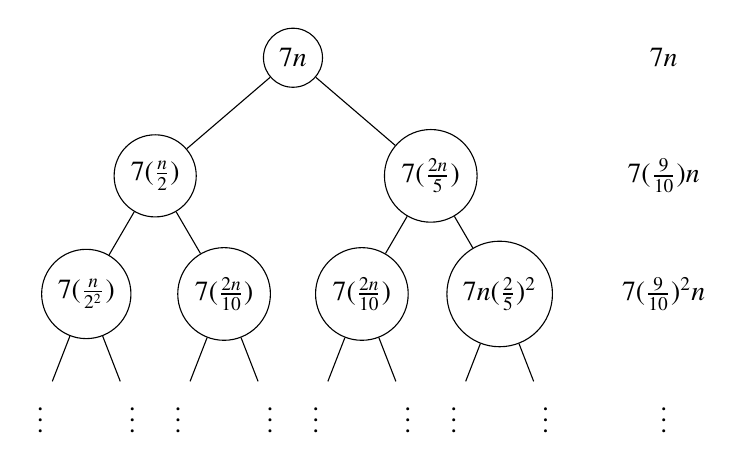
\begin{tikzpicture}[level/.style={sibling distance=35mm/#1}]
\node [circle,draw] (z){$7n$}
  child {node [circle,draw] (a) {$7(\frac{n}{2})$}
    child {node [circle,draw] (b) {$7(\frac{n}{2^2})$}
      child {node {$\vdots$}
      } 
      child {node {$\vdots$}}
    }
    child {node [circle,draw] (g) {$7(\frac{2n}{10})$}
      child {node {$\vdots$}}
      child {node {$\vdots$}}
    }
  }
  child {node [circle,draw] (j) {$7(\frac{2n}{5})$}
    child {node [circle,draw] (k) {$7(\frac{2n}{10})$}
      child {node {$\vdots$}}
      child {node {$\vdots$}}
    }
  child {node [circle,draw] (l) {$7n(\frac{2}{5})^2$}
    child {node {$\vdots$}}
    child {node (c){$\vdots$}
            child [grow=right] {node (r) {$\vdots$} edge from parent[draw=none]
              child [grow=up] {node (s) {$7(\frac{9}{10})^2 n$} edge from parent[draw=none]
                child [grow=up] {node (t) {$7(\frac{9}{10})n$} edge from parent[draw=none]
                  child [grow=up] {node (u) {$7n$} edge from parent[draw=none]}
                }
              }
            }
    }
  }
};

\end{tikzpicture}
\caption{Recurrence Tree} \label{fig:M1}
\end{figure}

Since, $\dfrac{n}{2}>\dfrac{2n}{5}$, So, the height of the rightmost subtree will determine the lower bound of the given recurrence, and the height of the leftmost subtree will determine the upper bound of the given recurrence.

Height of the leftmost subtree is : $\log_{2}n $ and so

\begin{align}
    T(n) &\leqslant 7n + 7(\frac{9}{10})n + 7(\frac{9}{10})^2 n + \dots + 7(\frac{9}{10})^{\log_{2}n} n \\
    T(n) &\leqslant 7n(1 + \frac{9}{10} + 7(\frac{9}{10})^2 + \dots + 7(\frac{9}{10})^{\log_{2}n}) \\
    T(n) &\leqslant 7n\dfrac{1-(\frac{9}{10})^{\log_{2} n + 1}}{1-\frac{9}{10}} \\
    T(n) &\leqslant 70n - 70n(n^{\log_{2}\frac{9}{10}} \frac{9}{10}) \\
    &= 70n - 63n^{0.85} \\
    \implies T(n) &\leqslant 70n\\
    \implies T(n) &\in \mathcal{O}(n)
\end{align}

Height of the rightmost subtree is :$log_{5/2}n$ and so,
\begin{align}
    T(n) &\geqslant 7n + 7(\frac{9}{10})n + 7(\frac{9}{10})^2 n + \dots + 7(\frac{9}{10})^{\log_{5/2}n} n \\
    T(n) &\geqslant 7n(1 + \frac{9}{10} + 7(\frac{9}{10})^2 + \dots + 7(\frac{9}{10})^{\log_{5/2}n}) \\
    T(n) &\geqslant 7n\dfrac{1-(\frac{9}{10})^{\log_{5/2} n + 1}}{1-\frac{9}{10}} \\
    T(n) &\geqslant 70n - 70n(n^{\log_{5/2}\frac{9}{10}} \frac{9}{10}) \\
    &= 70n - 63n^{0.89} \\
    T(n) &\geqslant n(70 - \frac{63}{n^{0.11}})
\end{align}
Since we consider complexity for large n,
$\lim_{n \to \infty} \frac{63}{n^{0.11}} = 0$
So $T(n) \geqslant 70n$

\section{Answer}
\begin{align}
\bullet T(n) \in \mathcal{O}(n) \\
\bullet T(n) \sim 70n
\end{align}
Hence option 3 is correct

\section{Verification}
To verify the theoretical results, I constructed a recursive function with given recurrence relation and measure the execution time for different n.

Here is the plot
\begin{figure}[!h]
    \centering
    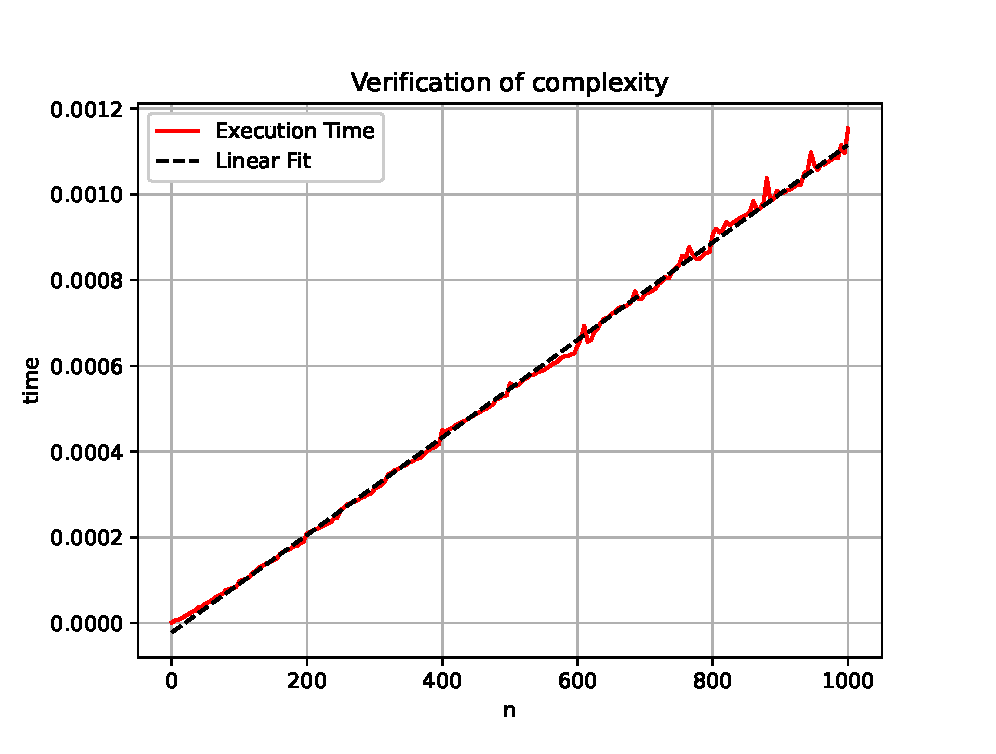
\includegraphics[scale=0.6]{figs/plot.eps}
    \caption{T(n) vs n}
    \label{fig:verification}
\end{figure}

We can clearly observe a linear curve. This verifies that 
$T(n) \in \mathcal{O}(n)$
\\
\\
This plot can be generated through the following python script
\begin{lstlisting}
https://github.com/aayush2710/EE4013-Assignment1/code/verification.py
\end{lstlisting}
\end{document}
